\chapter{Evaluierung}
\label{chap:evaluation}
Das vorliegende Kapitel befasst sich mit der Evaluierung des entwickelten Systems zur Strukturierung von \emph{Bedarfsmeldungen}. In dem Kapitel \ref{sec:literaturueberblick} wurde dargelegt, dass gängige Methoden zur Evaluierung von den einzelnen Information Retrieval Ansätzen und daraus entstehenden Pipelines und Hybriden die Methoden \emph{Precision, Recall} und \emph{F1-Score} angewendet werden. Grundsätzlich wäre dies ein valider Ansatz zur Evaluation. Dennoch bestehen keine Grundvoraussetzungen zur Durchführung dieser Methoden. Es liegt kein Datensatz mit ausreichenden Trainings und Testdaten vor. Die Erstellung eines Datensatzes auf Basis der originalen \emph{Bedarfsmeldungen} ist zeitaufwändig und erfordert Präzision. Dies ist im Rahmen der Ausarbeitung nicht weiter möglich. Stattdessen wird eine optimierende Evaluation auf Basis einer vordefinierten Erwartungshaltung durchgeführt, um Verbesserungspotenzial innerhalb des Systems zu ermitteln. Durch Modifikationen der Parameter der Pipeline wird versucht, eine vordefinierte Erwartungshaltung zu approximieren. 
%Des Weiteren wird die Dauer der Prozessschritte dokumentiert, um die Durchführungszeit der Anpassungen zu erfassen.

%nicht überlegen wie evaluieren sonder was will ich evaluieren,\\
%was sind die fragen die ich beantworten möchte, was sind die aussagen die ich machen will. hypothesen belegen, wiederlegen\\

%z.b. erwartungshaltung formulieren und mit cosine similarity gucken was näher dran ist,

%wie machen das andere ansätze,

%-------------------

%-was genau will ich in die evaluation packen, was will ich da machen? (nehme den vergleich mit llm raus)

\section{Versuchsdurchführung}
Der nachfolgende Versuch dient der Überprüfung der Ergebnisqualität des entwickelten Systems in Bezug auf die Strukturierung eines Volltextes in reduzierte Stichpunkte. Dazu wird eine synthetische Eingabe eines Skillfeldes einer \emph{Bedarfsmeldung} erstellt. Aus dieser wird manuell die wichtigsten Punkte auf Basis der Erkenntnisse aus Kapitel \ref{chap:erwartungshaltung} herausgearbeitet. Dieses dient als Erwartungshaltung, zu dem das System annäherungsweise gelangen soll. Zum semantischen Ähnlichkeitsvergleich wird die Kosinus-Ähnlichkeit verwendet. Dabei werden die Stichpunkte des Systems und der Erwartungshaltung vektorisiert und durch die Berechnung des \emph{Cosine-Similarity} ein Ähnlichkeitsscoring zwischen 0 und 1 ermittelt. Dabei spiegelt der Wert 0 eine niedrige und 1 eine hohe Ähnlichkeit wider. Das Ziel ist es die Schrittweise Anpassung der Parameter, den Ähnlichkeitswert näher zu 1 zu bringen. 
%Bei jedem Durchlauf des Systems wird die Durchlaufzeit gemessen, um Indikatoren für eine Längere Laufzeit zu ermitteln.
\paragraph{Word Embedding}\mbox{}\\
\emph{Word Embedding} sind Vektordarstellungen eines Wortes, die durch Training eines neuronalen Netzes auf einem großen Korpus gewonnen werden \cite{sitikhu2019comparison}. Sie finden häufig Anwendung bei der Klassifikation von Texten anhand semantischer Ähnlichkeit \cite{sitikhu2019comparison}. Word2vec stellt eine der am häufigsten verwendeten Formen von \emph{Word Embedding} dar \cite{sitikhu2019comparison}. Das Word2Vec-Modell nimmt einen Textkorpus als Eingabe und erzeugt Wortvektoren als Ausgabe, die anschließend für die Klassifizierung eines beliebigen anderen Wortes verwendet werden können \cite{sitikhu2019comparison}. Dazu wird der entsprechende Vektorwert ermittelt \cite{sitikhu2019comparison}. Im Rahmen des Experiments wurde ein vortrainiertes \emph{Word Embedding}-Modell namens \emph{ConceptNet Numberbatch} \cite{speer2017conceptnet} verwendet, um Vektoren für den Eingabetext zu erstellen.
\paragraph{Cosine-Similarity}\mbox{}\\
\emph{Cosine-Similarity} misst den Kosinus des Winkels zwischen zwei Vektoren, die auf eine mehrdimensionale Ebene projiziert werden \cite{sitikhu2019comparison}. Es stellt eine weit verbreitete Metrik im Bereich des Information Retrieval dar \cite{rahutomo2012semantic}. Die Metrik modelliert ein Textdokument als einen Vektor von Begriffen \cite{rahutomo2012semantic}. Die Berechnung des Kosinuswerts zwischen den Vektoren zweier Dokumente erlaubt die Ermittlung der Ähnlichkeit zwischen diesen Dokumenten \cite{rahutomo2012semantic}. Der Grad der Ähnlichkeit zwischen den Vektoren ist ein Indikator für die Relevanz zwischen den Texten \cite{rahutomo2012semantic}.
%Die Cosinus-Ähnlichkeit ist jedoch nicht in der Lage, die semantische Bedeutung des Textes adäquat zu erfassen. 
%Die syntaktische Implementierung der Cosinus-Ähnlichkeitsmessung zwischen zwei Vektoren kann mitunter zu unzuverlässigen Ergebnissen führen. Der Syntaxabgleich ist möglicherweise nicht in der Lage, das Problem der unterschiedlichen semantischen Bedeutung zu lösen. Dies kann zu falschen Ergebnissen und einer Verschlechterung der Leistung des Information Retrieval Systems führen.
\paragraph{Optimierungsmaßnahmen}\label{sec:optimierungsmaßnahmen}\mbox{}\\
Im Rahmen der Evaluierung erfolgt eine schrittweise Anpassung der vier Parameter des Systems. Im Anschluss an jede Anpassung erfolgt eine Evaluierung der Cosine-Similarity im Hinblick auf eine etwaige Verbesserung oder Verschlechterung im Vergleich zur Erwartungshaltung. Im Anschluss an die Ermittlung des höchsten Scores werden die Ergebnisse dargestellt und Auffälligkeiten diskutiert. Zum Schluss jedes Schrittes erfolgt eine feste Übernahme des betreffenden Parameters in das System. In der Folge wird der darauffolgende Parameter angepasst. Die vier zu evaluierenden Parameter sind wie folgt definiert:
\begin{enumerate}
	\item \textbf{Korpusgröße der Schlüsselwortextraktion} \\ In diesem Zusammenhang erfolgt eine Anpassung der Menge an \emph{Bedarfsmeldungen} als Korpus für die Schlüsselwortextraktion. In einem nächsten Schritt werden neben den \emph{offenen} und \emph{eskalierten} \emph{Bedarfsmeldungen} auch alle bereits \emph{geschlossenen} Bedarfsmeldungen in den Korpus aufgenommen. Dies resultiert in einer signifikanten Erhöhung der Wortmenge innerhalb von \emph{TF-IDF}. Im Rahmen der Evaluierung wird untersucht, ob die Erweiterung des Korpus einen positiven Effekt auf die Identifikation der Schlüsselwörter hat.
	\item \textbf{Scorethreshold} \\ Innerhalb der \emph{TF-IDF} erfolgt eine Anpassung des Scorethresholds zur Ausschließung von Schlüsselwörtern mit geringem Score. Der Score wird zunächst mit einem niedrigen Wert (nahe 0) getestet und anschließend schrittweise erhöht.
	\item \textbf{POS-Tagging Kombinationen erlauben} \\ Im Rahmen dieses Prozesses erfolgt eine schrittweise Freigabe von Wortartenkombinationen, die als untypisch definiert wurden. Im Rahmen dieses Prozesses wird in jedem Schritt eine Kombination aus dem System entfernt, bis schließlich keine Kombinationen mehr enthalten sind.
	\item \textbf{Übersetzung beibehalten} \\ Im Rahmen der Untersuchung werden die einzelnen Übersetzungsschritte entfernt und deren Einfluss auf die Ergebnisqualität evaluiert.
\end{enumerate}
%pareto evaluation --> ziel ist es die pareto ebene zu finden. Einfach aufschreiben. 80 20 prinzip --> ich habe versucht mit 5 stellschrauben und habe eine qualitätsmetrik(zahl 0-1) ich drehe ein qualitätsmerkmal dann verbessert sich zahl. Fixiere die stellschrauben und mache weiter --> bis ich alles durch habe --> optimierende evaluation (linear)
\paragraph{Systemspezifikation}\mbox{}\\
%Die Zeitmessung spielt in der Hinsicht eine Rolle als, dass langfristig eine Lösung gesucht wird, die \emph{Bedarfsmeldungen} in Echtzeit bearbeiten kann. Bei der Messung in dieser Evaluation gilt es daher Ausreißer zu identifizieren, die bei Veränderungen der Parameter für eine erhebliche zeitliche Erhöhung sorgen. Für die Zeitmessung wird vor dem Aufruf des ersten und nach dem letzten Schritt im System jeweils ein Zeitstempel angelegt. Dazu wird die Bibliothek \emph{time} verwendet. Die Zeitstempel werden generiert und in Variablen zwischengespeichert. Zum Schluss wird die Differenz aus beiden Zeitstempeln ermittelt, in Sekunden umgerechnet und ausgegeben. 
Im Rahmen der Evaluation wurde ein System eingesetzt, dessen Spezifikationen wie folgt definiert sind: Prozessor: 13th Gen Intel(R) Core(TM) i7-1360P, 2200 MHz, 12 Kerne, 16 logische Prozessoren, RAM: 16 GB
\section{Beschreibung des verwendeten Datensatzes}
In diesem Kapitel wird zunächst eine Ausgangslage konstruiert, auf deren Basis anschließend eine Erwartungshaltung definiert wird. Die Berechnung der Kosinus-Ähnlichkeit erfolgt mit dem Ziel, eine Verbesserung der textuellen Ähnlichkeit festzustellen.
\paragraph{Ausgangslage}\mbox{}\\
Die Ausgangslage bildet ein synthetischer Datensatz. Die Grundlage hierfür bildeten authentische \emph{Bedarfsmeldungen}. Bei der Erstellung wurde darauf geachtet, dass der Datensatz einer echten \emph{Bedarfsmeldung} ähnelt. Der Ausgangsdatenbestand liegt als Volltext vor.\\

\textbf{Aufgabe ist es, beim Aufbau einer Plattform zu unterstützen, die auf Basis von Azure, OpenAI, Java und ReactJS aufgebaut ist. Aktuell (und perspektivisch) haben wir einen Engpass vor allem im Frontend. Hilfe im Backend (Java) wäre aber auch willkommen.\textbackslash r\textbackslash nDas Projekt bietet einiges an Potenzial, d.h. wir erwarten hier noch einige Interessenten für die Plattform. 2 Jahre Erfahrung und Kenntnisse in der Software-Entwicklung mit Java sind erwünscht}\\

Der Volltext weist eine Vielzahl unterschiedlicher Zeichen, Formatierungen (beispielsweise \textbackslash r \textbackslash n für Zeilenumbrüche) sowie zeitbezogene Daten auf.
\paragraph{Erwartungshaltung}\mbox{}\\
Die Erwartungshaltung wurde manuell aus der Ausgangslage abgeleitet. Bei der Erstellung wurde darauf geachtet, dass Füllwörter entfernt und wichtige Informationen beibehalten wurden, die in Kapitel \ref{chap:erwartungshaltung} erfasst wurden. Das Ziel besteht in der Annäherung an die Erwartungshaltung.
\begin{itemize}
	\itemsep-0.5em
	\item Aufbau einer Plattform
	\item Azure, OpenAI, Java und ReactJS
	\item Engpass im Frontend
	\item Hilfe im Backend (Java)
	\item bietet Potenzial
	\item erwarten Interessenten für Plattform.
	\item 2 Jahre Erfahrung in Java
\end{itemize}
\section{Präsentation und Diskussion der Ergebnisse}
Im Folgenden werden die Resultate der einzelnen Anpassungsschritte, wie sie in Kapitel \ref{sec:optimierungsmaßnahmen} beschrieben sind, dargelegt.
\paragraph{1. Korpusgröße der Schlüsselwortextraktion}\mbox{}\\
Die These besagt, dass mit einer Zunahme der im Textkorpus enthaltenen Wörter und Daten für die Schlüsselwortextraktion eine Steigerung der Qualität der Schlüsselwörter einhergeht. Diese Annahme basiert auf der Prämisse, dass eine höhere Anzahl an themenbezogenen Dokumenten, die häufig verwendete fachliche Ausdrücke enthalten, zu einer höheren Gewichtung dieser Ausdrücke bei der Term-Frequency-Berechnung führt. Dies wiederum resultiert in einer höheren Wahrscheinlichkeit, dass sie als potenziell wichtige Schlüsselwörter identifiziert werden.\\

Die zuvor aufgestellte These soll durch eine schrittweise Erhöhung der Anzahl der im Textkorpus enthaltenen Wörter überprüft werden. Dazu wird die \emph{TF-IDF}-Methode eingesetzt. Die Bedarfsmeldungen mit den Status \emph{offen}, \emph{eskaliert} und \emph{angeboten} wurden gemäß der Vorverarbeitung in Kapitel \ref{tfidf} zu Textblöcken mit Wörtern zusammengefasst. Die ersten zehn Wörter der \emph{offenen Bedarfsmeldungen} dienen als Grundlage für die weitere Analyse. Im Rahmen der Analyse werden den \emph{Bedarfsmeldungen} sukzessive mehr Wörter hinzugefügt, um die Veränderung des Scores zu beobachten. Bei der Durchführung ist der Scorethreshold bei 0.0, um Einflüsse vor den Anpassungen in Schritt 2 zu vermeiden.
\begin{figure}[H]
	\centering  
	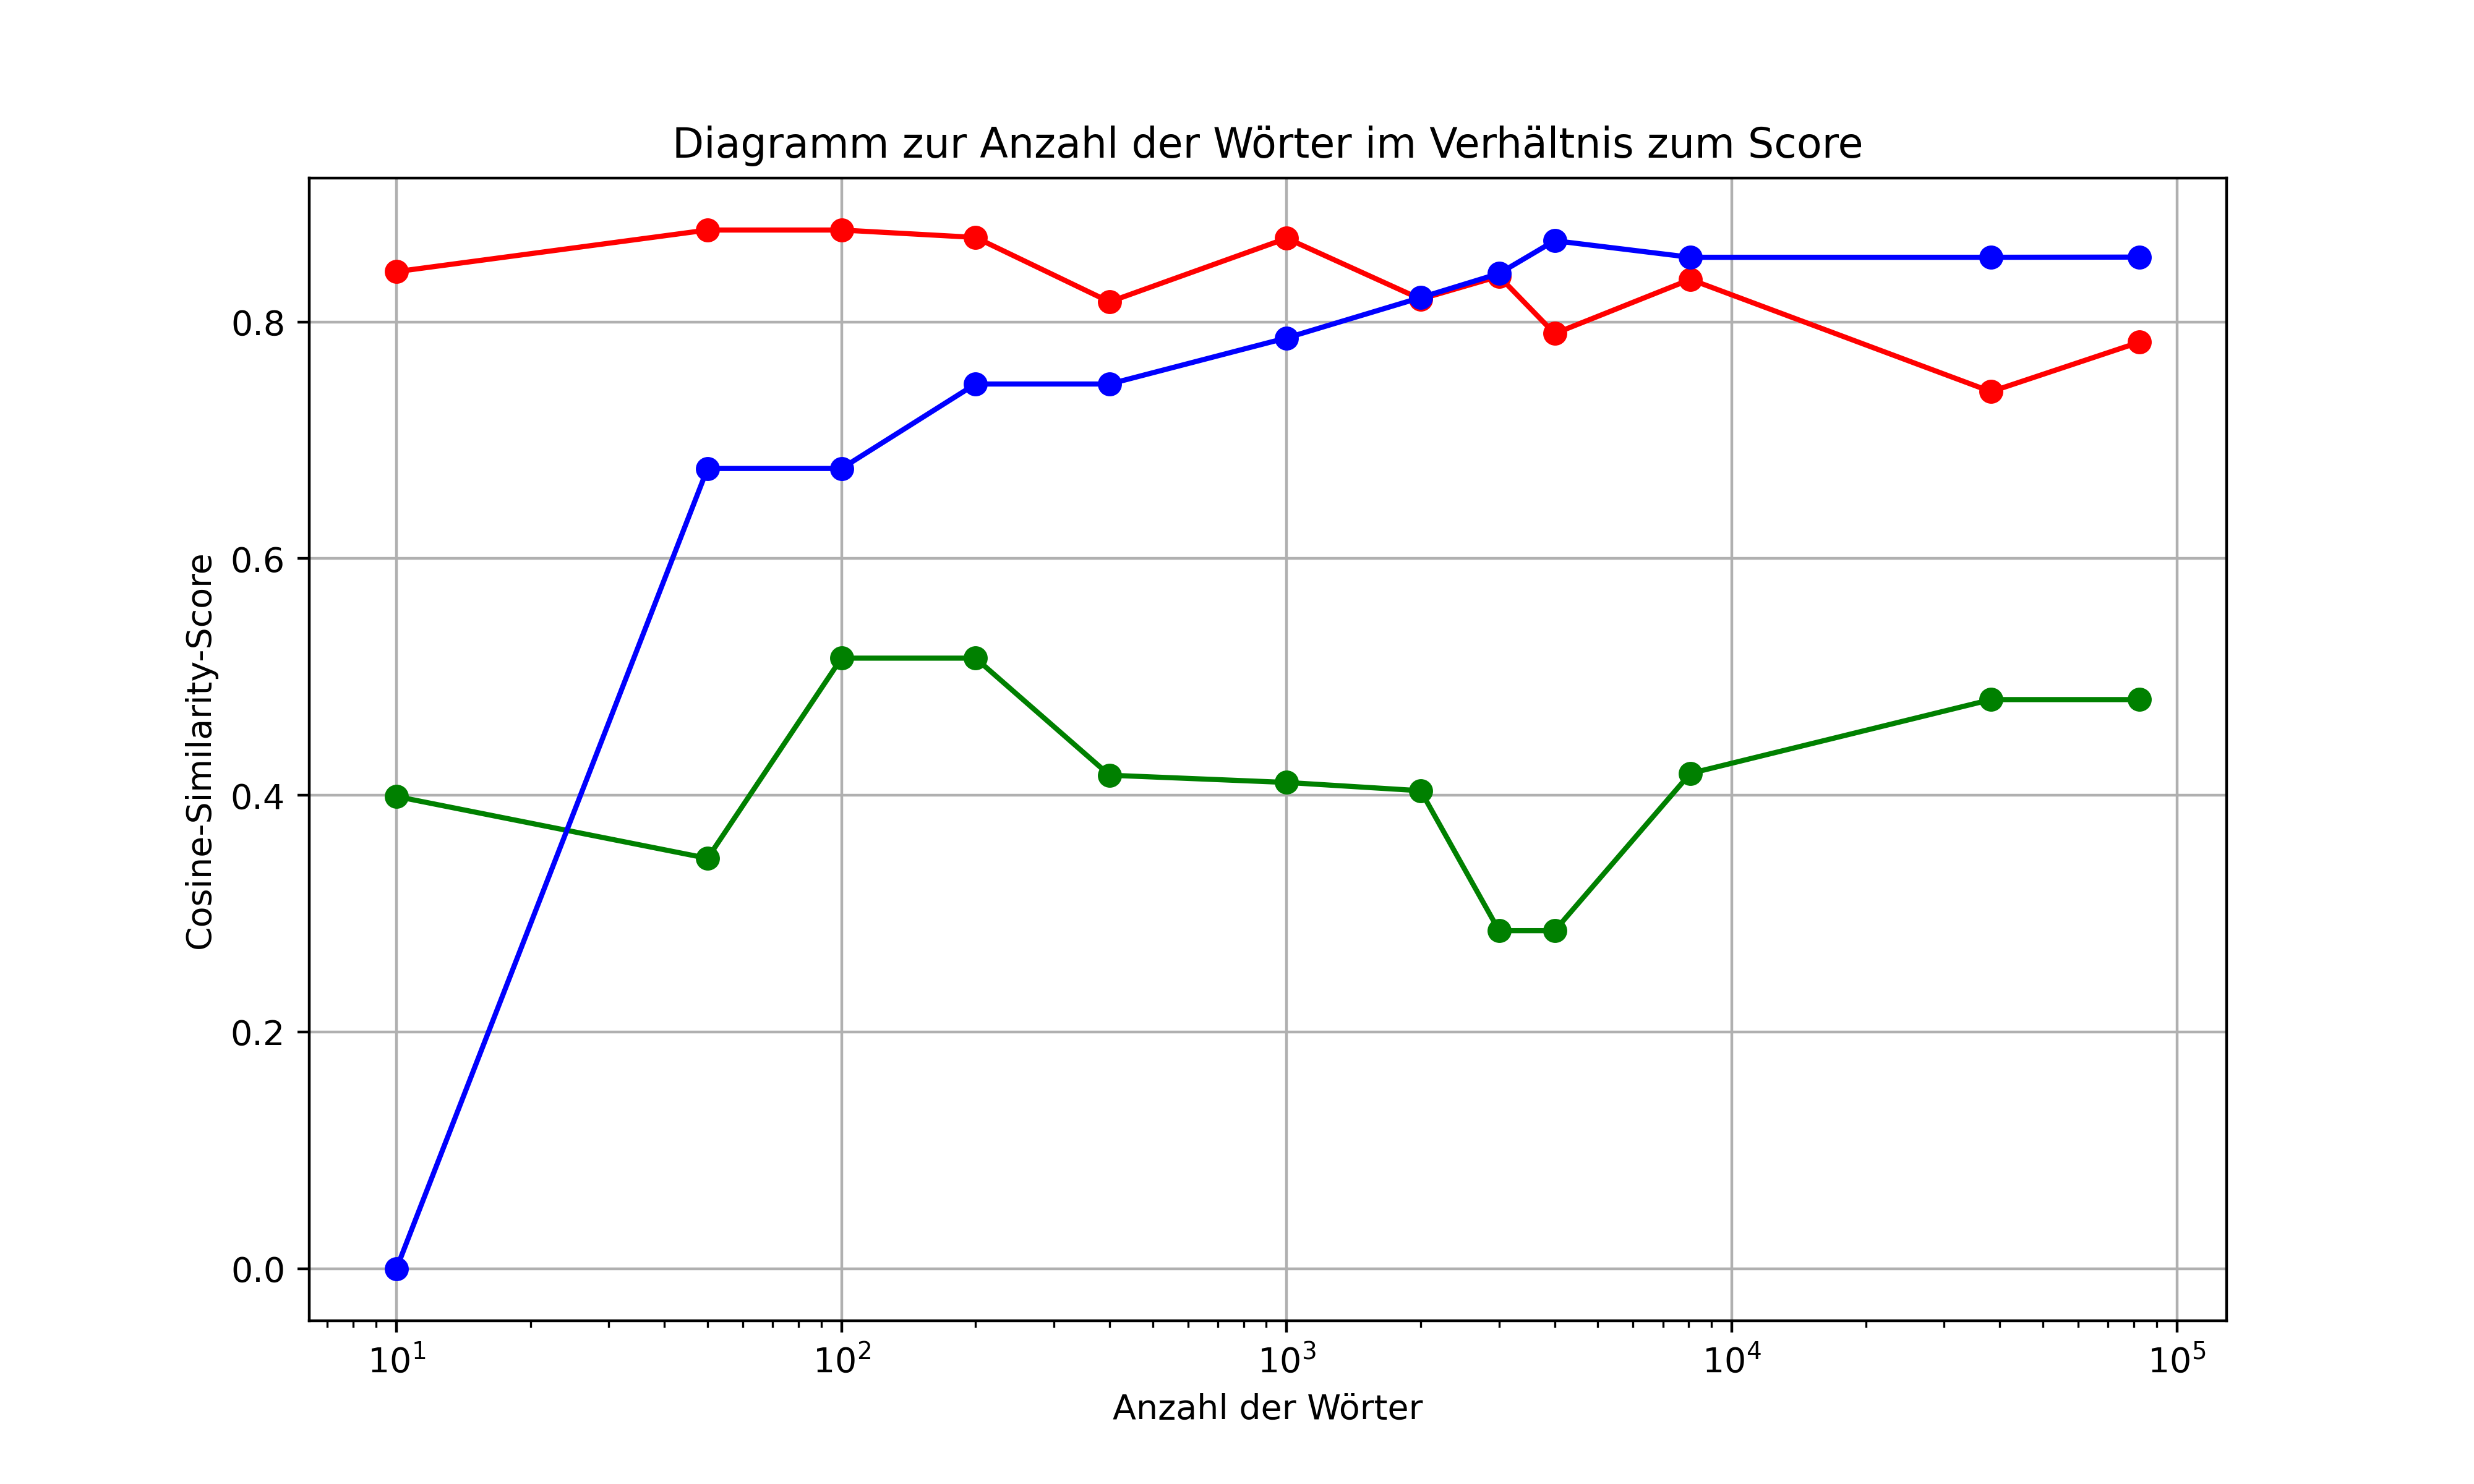
\includegraphics[width=\linewidth]{plot/e1-woerter-score.png}
	\caption{Diagramm zur Anzahl der Wörter im Verhältnis zum Score.}
	\label{fig:woertervsscore}
\end{figure}\mbox{} \\
In der Abbildung \ref{fig:woertervsscore} wird das Verhältnis der Anzahl an Wörtern zum Score in Form eines Diagramms dargestellt. Im halblogarithmischen Diagramm lässt sich ein annähernd linearer Zusammenhang zwischen dem Score und der Anzahl der Wörter erkennen. Dies impliziert, dass der Score proportional zur exponentiellen Anzahl der Wörter ist. Der beschriebene Effekt ist bis zum Erreichen eines Plateaus bei 80.000 Wörtern erkennbar. In der Konsequenz lässt sich ein Anstieg der Ergebnisqualität bis zu einem gewissen Punkt feststellen, je mehr Wörter im Textkorpus enthalten sind. Eine Überschreitung dieses Punktes führt zu einer Stagnation der Ergebnisqualität. Bei einer zu geringen Anzahl an Wörtern im Textkorpus (n < 10) konnten keine Scoring-Werte generiert werden. Die Generierung von Stichpunkten durch das System ist nur möglich, wenn die entsprechenden Schlüsselwörter vorhanden sind, da andernfalls keine Zuordnung erfolgen kann.
\begin{center}
	\begin{tabularx}{1\textwidth} { 
			| >{\raggedright\arraybackslash}X 
			|| >{\raggedright\arraybackslash}X | }
		\hline
		Anzahl Wörter: 4000
		& Anzahl Wörter: 8070 \\
		\hline
		\begin{itemize}[topsep=0pt]
			\itemsep-0.5em
			\item die Aufgabe Unterstützung Entwicklung Plattform basierend auf Azure OpenAI
			\item OpenAI, Java, ReactJS
			\item reactjs Zukunft
			\item zukünftiger Engpass
			\item Engpass vor allem Frontend Hilfe Backend Java wäre willkommen
			\item begrüßen das Projekt viel Potenzial dh
			\item d.h. interessiert
			\item Interessenten Plattform Erfahrung Kenntnisse Software Entwicklung Java erwünscht
			\item 2 Jahre
		\end{itemize} & \begin{itemize}[topsep=0pt]
			\itemsep-0.5em
			\item die Aufgabe Unterstützung Entwicklung Plattform basierend auf Azure OpenAI
			\item OpenAI, Java, ReactJS
			\item reactjs Zukunft
			\item zukünftiger Engpass
			\item Engpass vor allem Frontend Hilfe Backend Java wäre willkommen
			\item begrüßen das Projekt viel Potenzial dh interessiert
			\item Interessenten Plattform Erfahrung Kenntnisse Software Entwicklung Java erwünscht
			\item 2 Jahre
		\end{itemize}\\
		\hline
	\end{tabularx}\\
	\captionof{table}{Gegenüberstellung der Ergebnisse mit 4000 und 8070 Wörtern im Textkorpus.}
	\label{tab:gegenüberstellung-e1}
\end{center}
In der Tabelle \ref{tab:gegenüberstellung-e1} erfolgt eine Gegenüberstellung der Ergebnisse bei einer Wortanzahl von 4.000 bzw. 8.0070 Wörtern. In der linken Spalte findet sich das Resultat mit dem höchsten Score. Das darauffolgende Ergebnis in der rechten Spalte ist Bestandteil des beobachteten Plateaus. Der Unterschied zwischen den beiden Resultaten manifestiert sich in der linken Spalte, Punkt 7, beim Stichwort \emph{d. h. interessiert}. Dieses ist auf der rechten Seite der Tabelle in Punkt 6 zu finden. Der Unterschied ist marginal, sodass der Beginn der Plateaus ab 8070 Wörtern als Anhaltspunkt für die weitere Evaluation verwendet werden kann.
\paragraph{2. Scorethreshold}\mbox{}\\
Die vorliegende These beschreibt, dass die Qualität von Schlüsselwörtern durch einen Threshold-Parameter optimiert werden kann. Wörter, die den Threshold unterschreiten, werden bei der Ermittlung der Schlüsselwörter nicht berücksichtigt, wodurch Wörter mit einem niedrigen Scoring keine Berücksichtigung finden. Ein niedriger Score kann darauf hinweisen, dass ein Wort lediglich einmalig im Kontext vorkommt und folglich kein Schlüsselwort darstellt.\\

Die zuvor aufgestellte These soll im Folgenden einer Überprüfung unterzogen werden. Zu diesem Zweck werden die Threshold-Werte in Intervallen von 0,0 bis 1,0 in Schritten von 0,01 durchlaufen.
\begin{figure}[H]
	\centering  
	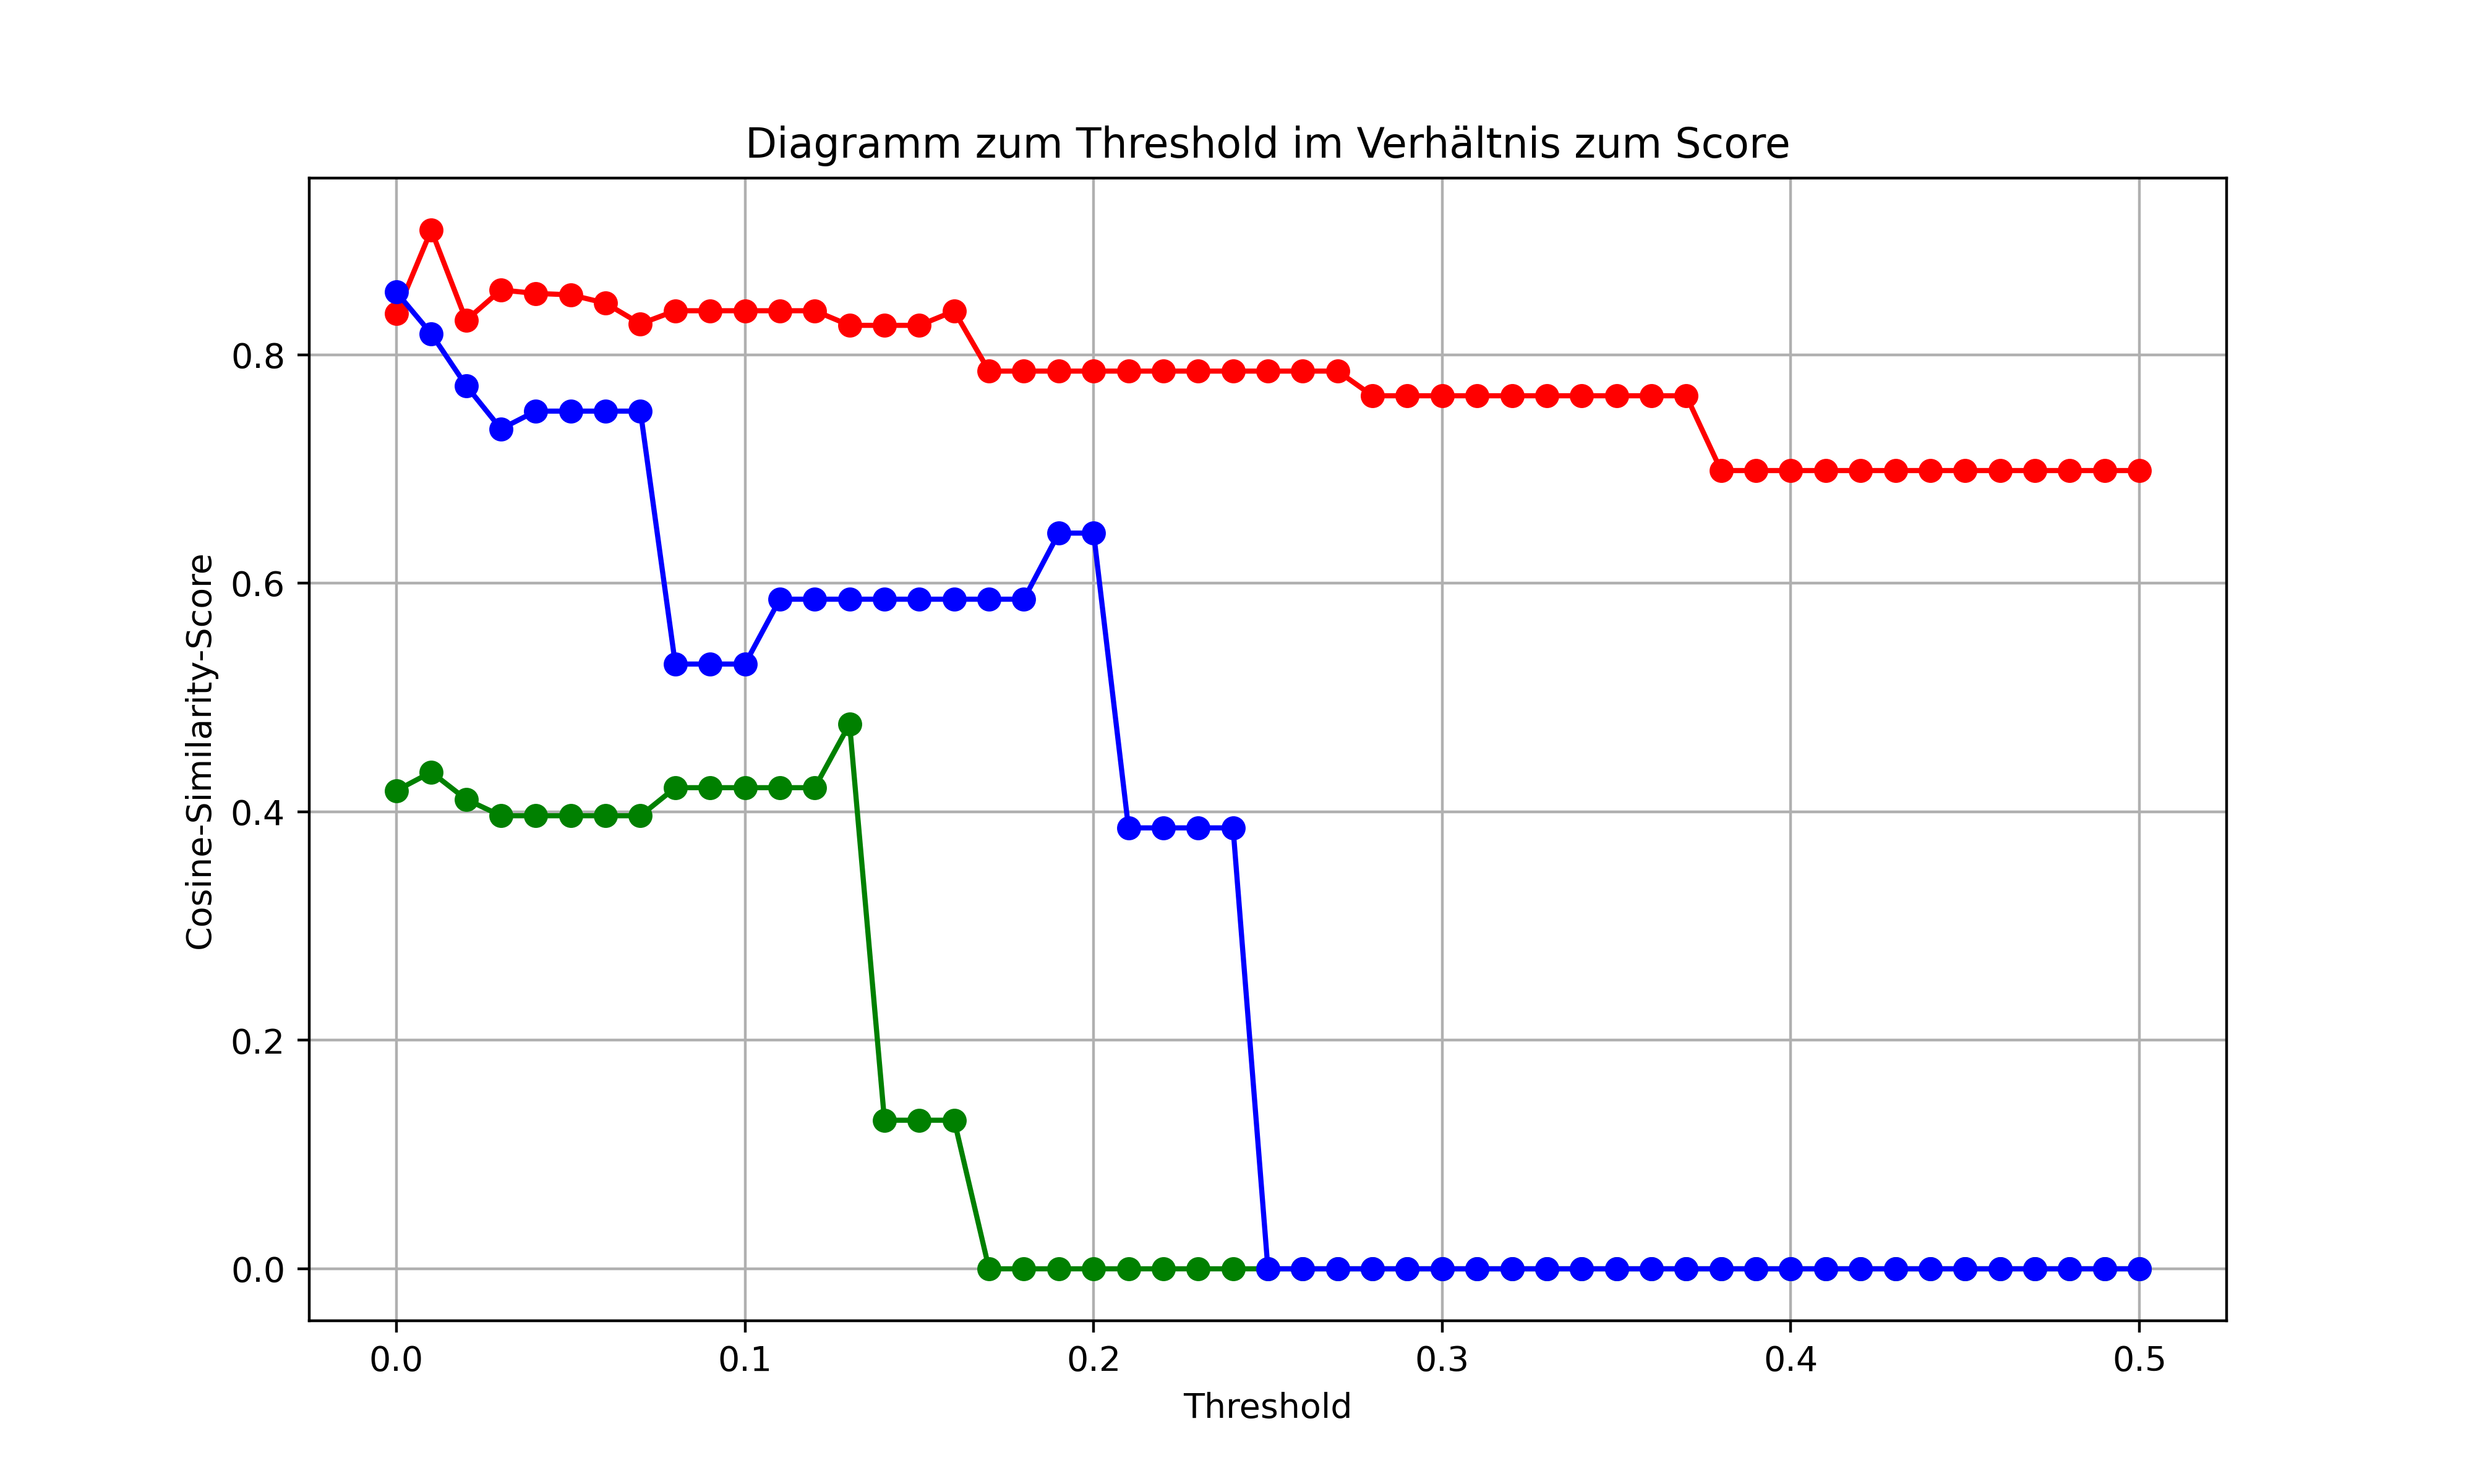
\includegraphics[width=\linewidth]{plot/e2-threshold-score.png}
	\caption{Diagramm zum Threshold im Verhältnis zum Score.}
	\label{fig:thresholdvsscore}
\end{figure}\mbox{} \\
In der Abbildung \ref{fig:thresholdvsscore} ist das Diagramm dargestellt, das die Thresholds im Verhältnis zum Score widerspiegelt. Die dargestellten 0,01-Schritte genügen, um einen Abwärtstrend zu identifizieren. Die aufgestellte These ist als falsch zu erachten, da bei einer Erhöhung des Thresholds der Score annähernd linear sinkt. Dies geschieht bis zum Threshold-Wert 0.24. Ein darüber hinausgehender Wert entfernt zu viele Wörter aus der Schlüsselwortermittlung, wodurch keine Stichpunkte gebildet werden und der Score den Wert 0 annimmt. Der höchste Thresholdwert des Diagramms der Abbildung \ref{fig:thresholdvsscore} wurde auf den Wert 0.5 gesetzt, da alles darüber hinaus ebenfalls den Similarity-Score 0 annehmen.
\begin{center}
	\begin{tabularx}{1\textwidth} { 
			| >{\raggedright\arraybackslash}X 
			|| >{\raggedright\arraybackslash}X | }
		\hline
		Threshold: 0.0
		& Threshold: 0.05 \\
		\hline
		\begin{itemize}[topsep=0pt]
			\itemsep-0.5em
			\item die Aufgabe Unterstützung Entwicklung Plattform basierend auf Azure OpenAI
			\item OpenAI, Java, ReactJS
			\item reactjs Zukunft
			\item zukünftiger Engpass
			\item Engpass vor allem Frontend Hilfe Backend Java wäre willkommen
			\item begrüßen das Projekt viel Potenzial dh interessiert
			\item Interessenten Plattform Erfahrung Kenntnisse Software Entwicklung Java erwünscht
			\item 2 Jahre
		\end{itemize} & \begin{itemize}[topsep=0pt]
		\itemsep-0.5em
		\item die Aufgabe
		\item Entwicklungsplattform zur Aufgabenunterstützung
		\item OpenAI, Java, ReactJS
		\item Backend Java würde
		\item begrüßen das Projekt Los
		\item Plattformerfahrung Kenntnisse Softwareentwicklung Java erwünscht
		\item 2 Jahre
		\end{itemize}\\
		\hline
	\end{tabularx}\\
	\captionof{table}{Gegenüberstellung der Ergebnisse mit dem Threshold 0.0 und 0.05.}
	\label{tab:gegenüberstellung-e2}
\end{center}
Eine manuelle Betrachtung der Ergebnisse hat gezeigt, dass ohne die Anwendung eines Thresholds eine deutliche Zunahme der Stichpunktlänge von 2-5 Wörtern pro Stichpunkt zu 2-9 Wörtern pro Stichpunkt zu verzeichnen ist. Dies ist in Tabelle \ref{tab:gegenüberstellung-e2} durch die Ergebnisse mit den Thresholds 0.0 und 0.05 dargestellt. Die Inhalte der Stichpunkte sind von hoher Relevanz, was zu einem entsprechend hohen Score führt. Dennoch kann ein geringer Threshold einen positiven Effekt auf die Stichpunkte ausüben auch wenn der Score dadurch leicht abfällt. Der direkte manuelle Vergleich hat ergeben, dass für die ausgewählte Ausgangslage ein Score im Bereich von 0.04 bis 0.07 die Stichpunkte verkürzt werden, ohne die wichtigen Informationen zu beeinträchtigen. Somit kann für die weitere Evaluation der Wert 0.05 aus der Gegenüberstellung weiter verwendet werden.
\paragraph{3. POS-Tagging Kombinationen erlauben}\mbox{}\\
Die hier vorgestellte These besagt, dass die Qualität der Stichpunkte durch die Entfernung von untypischen Wortkombinationen beeinträchtigt wird. Durch fehlende Entfernung untypischer Wortkombinationen könnten Stichpunkte entstehen, die inhaltlich eine geringere Kohärenz beinhalten und dadurch auch einen geringeren Score erhalten.\\

Die in Kapitel \ref{postagging} präsentierte Liste mit POS-Tagging-Kombinationen wird im Folgenden schrittweise modifiziert, um die zugrundeliegende These zu überprüfen.
\begin{figure}[H]
	\centering  
	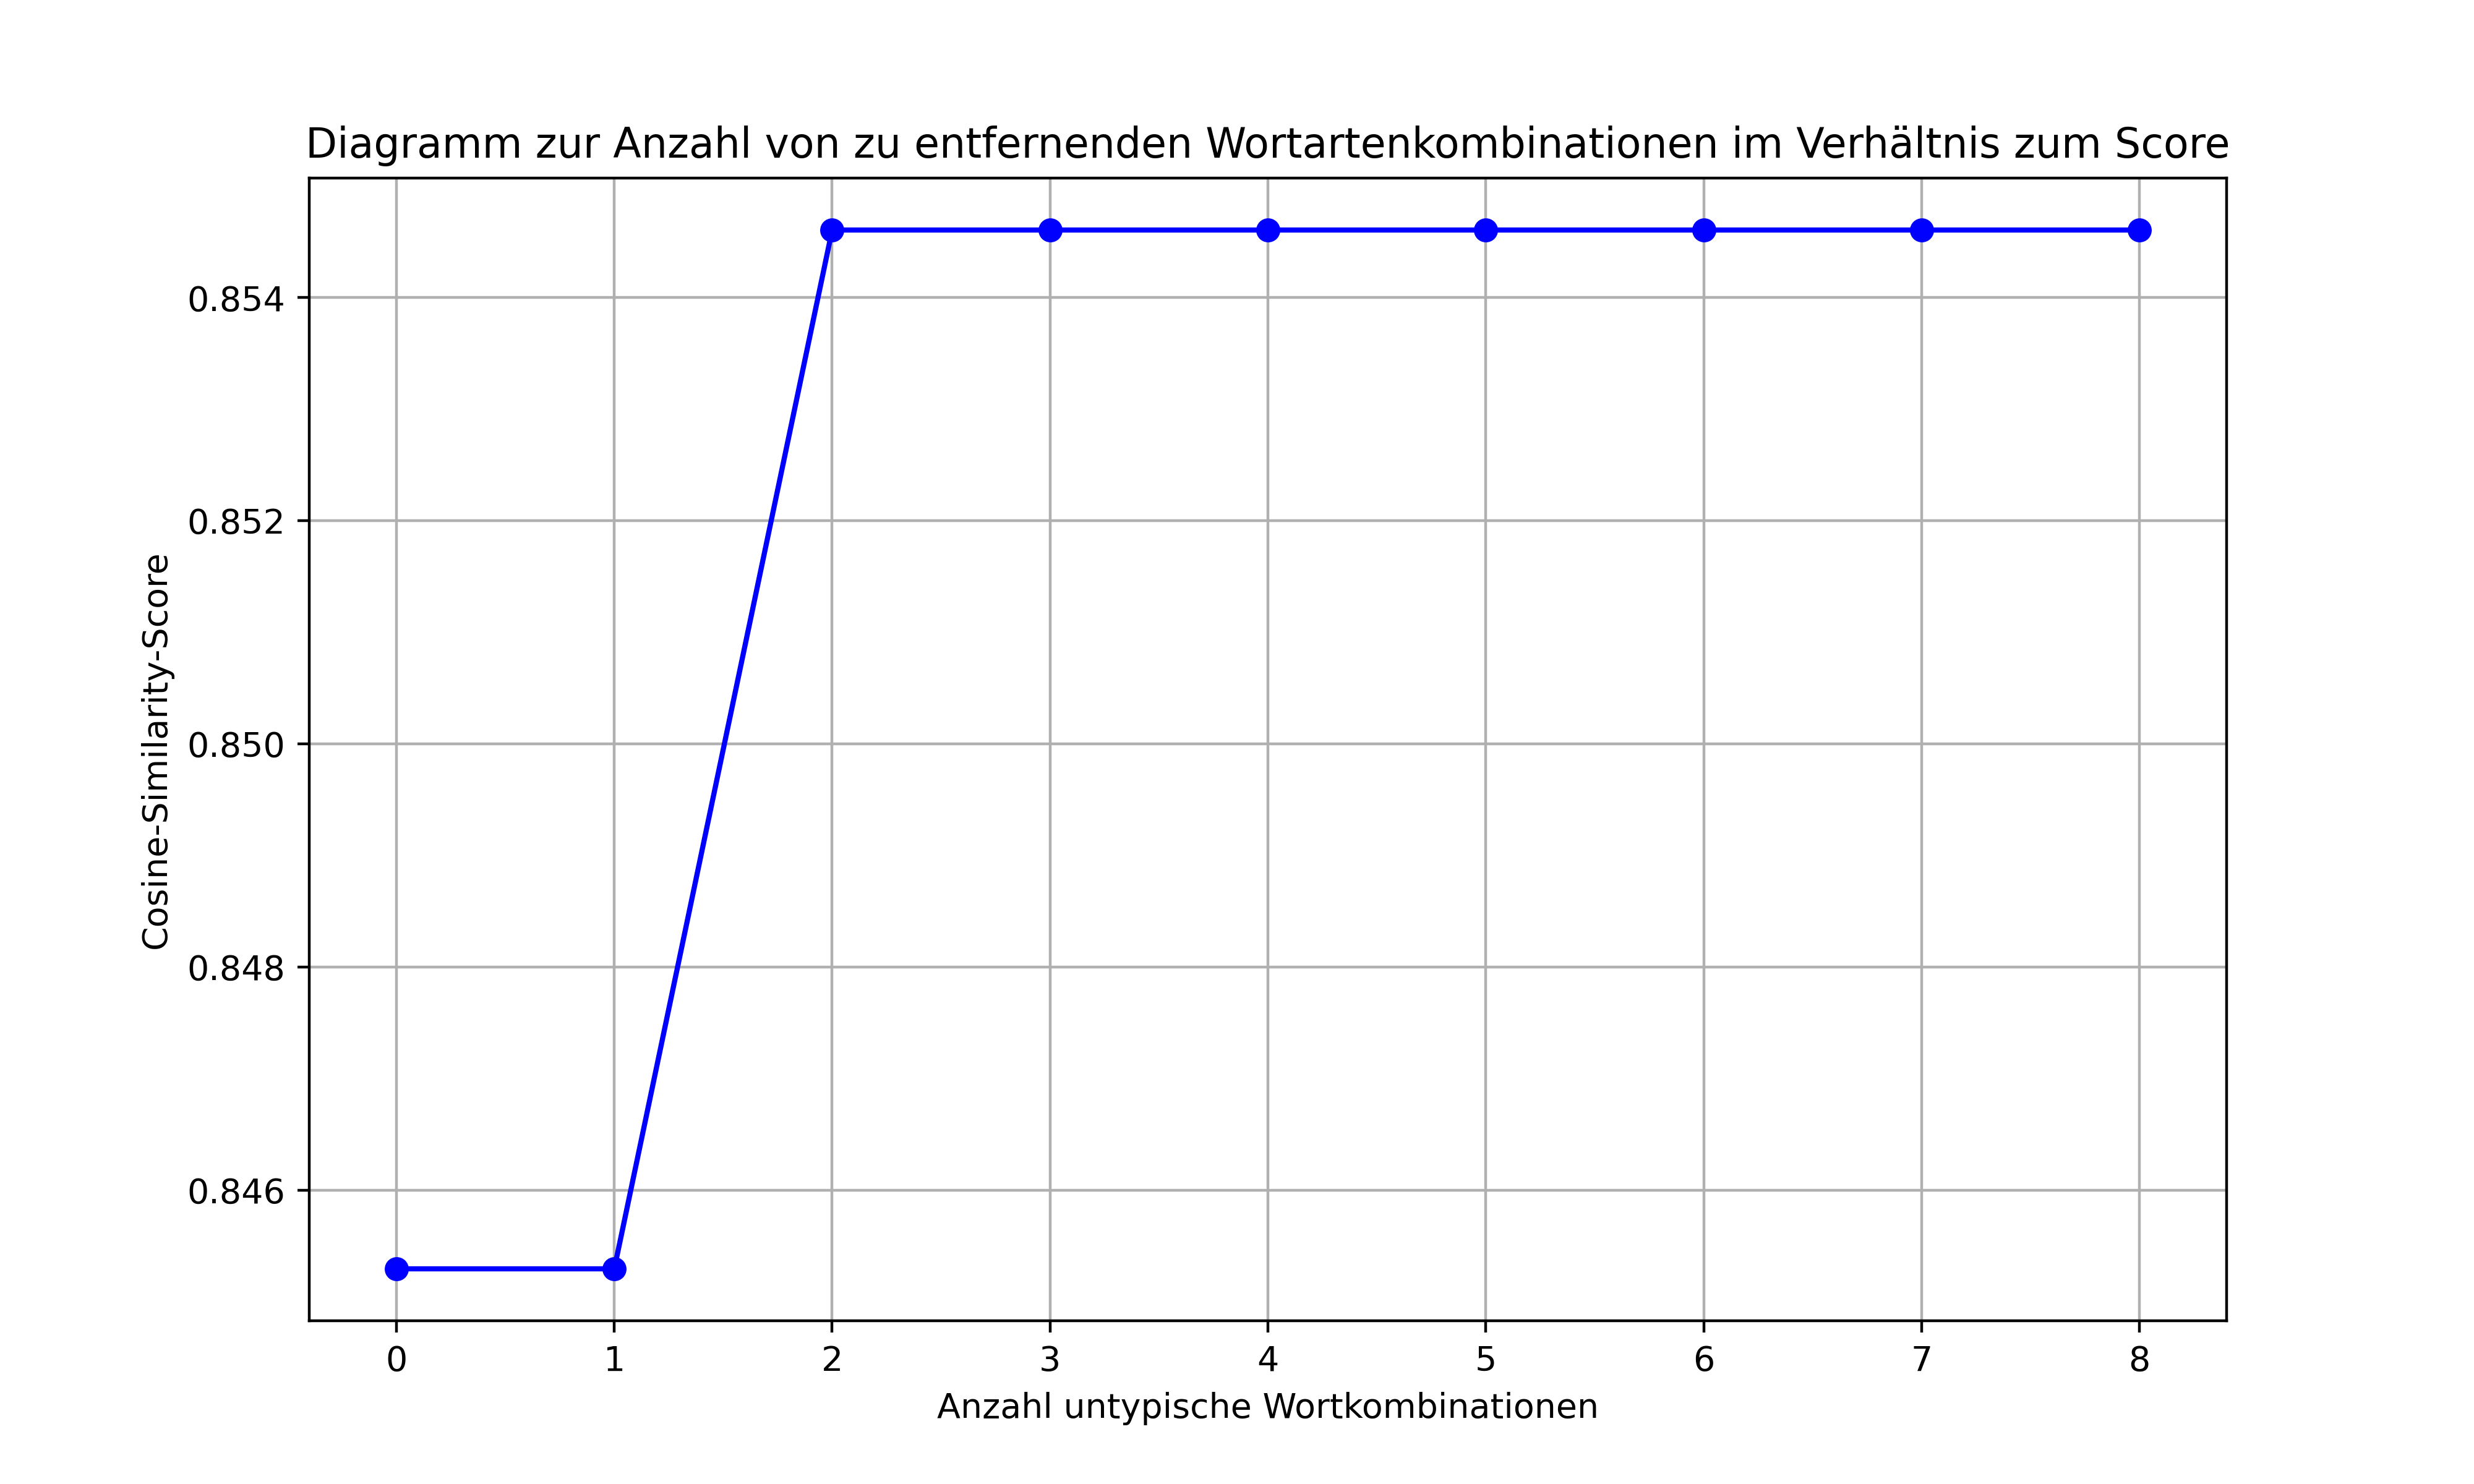
\includegraphics[width=\linewidth]{plot/e3-wortkombinationen-score.png}
	\caption{Diagramm zur Anzahl von zu entfernenden Wortartenkombinationen im Verhältnis zum Score.}
	\label{fig:wordcombinationvsscore}
\end{figure}\mbox{} \\
In der Abbildung \ref{fig:wordcombinationvsscore} ist das Diagramm zur Anzahl der zu entfernenden Wortartenkombinationen im Verhältnis zum Score dargestellt. Die Werte auf der X-Achse quantifizieren die Anzahl der enthaltenen Wortkombinationen. Der Wert 0 entspricht der Durchführung des Systems ohne den Schritt der Entfernung von untypischen Wortkombinationen. Der Wert 8 stellt demgemäß den Schritt dar, bei dem sämtliche acht Kombinationen aus der Tabelle \ref{tab:wortkombinationen} aus dem Kapitel \ref{postagging} in die Auswertung einbezogen sind. Die Werte dazwischen repräsentieren die jeweilige Anzahl der zu dem Zeitpunkt enthaltenen Kombinationen. 
\begin{center}
	\begin{tabularx}{1\textwidth} { 
			| >{\raggedright\arraybackslash}X 
			|| >{\raggedright\arraybackslash}X | }
		\hline
		Anz. untypischer Wortkombinationen: 1
		& Anz. untypischer Wortkombinationen: 2 \\
		\hline
		\begin{itemize}[topsep=0pt]
			\itemsep-0.5em
			\item die Aufgabe
			\item Entwicklungsplattform zur Aufgabenunterstützung
			\item OpenAI, Java, ReactJS
			\item Backend Java würde
			\item begrüßen das Projekt Los
			\item Plattformerfahrung Kenntnisse Softwareentwicklung Java erwünscht
			\item 2 Jahre
		\end{itemize} & \begin{itemize}[topsep=0pt]
			\itemsep-0.5em
			\item 
		\end{itemize}\\
		\hline
	\end{tabularx}\\
	\captionof{table}{Gegenüberstellung der Ergebnisse mit 1 und 2 untypischen Wortkombinationen.}
	\label{tab:gegenüberstellung-e3}
\end{center}
Es lässt sich erkennen, dass sich der Score von 0,84529346 auf 0,85460645 verbessert hat, nachdem im Schritt 2 die zu entfernende Kombination aus Verb und Adjektiv hinzugefügt wurde. Dies belegt, dass die aufgestellte These korrekt ist und das System durch die Entfernung untypischer Wortkombinationen ein besseres Ergebnis liefert.
\todo{nochmal gucken. Kann die Werte nicht mehr reproduzieren}
\paragraph{4. Übersetzung beibehalten}\mbox{}\\
Die These lautet, dass die implementierten Ansätze ohne eine Übersetzung ins Englische zu schlechteren Ergebnissen führen. Die These basiert auf der Annahme, dass die Modelle mit englischen Datensätzen trainiert wurden und daher bei der Anwendung auf deutsche Wörter möglicherweise nicht die optimalen Ergebnisse liefern.\\

\begin{center}
	\begin{tabularx}{1\textwidth} { 
			| >{\raggedright\arraybackslash}X 
			|| >{\raggedright\arraybackslash}X | }
		\hline
		mit Übersetzung
		& ohne Übersetzung \\
		\hline
		Score: 0.75364363
		& Score: 0.7852247 \\
		\hline
		\begin{itemize}[topsep=0pt]
			\itemsep-0.5em
			\item die Aufgabe
			\item Entwicklungsplattform zur Aufgabenunterstützung
			\item OpenAI, Java, ReactJS
			\item Backend Java würde
			\item begrüßen das Projekt Los
			\item Plattformerfahrung Kenntnisse Softwareentwicklung Java erwünscht
			\item 2 Jahre
		\end{itemize} & \begin{itemize}[topsep=0pt]
			\itemsep-0.5em
			\item openai java und
			\item backend java wäre
			\item mit java sind
		\end{itemize}\\
		\hline
	\end{tabularx}\\
	\captionof{table}{Gegenüberstellung der Ergebnisse mit und ohne Übersetzungsschritt.}
	\label{tab:gegenüberstellung-e4}
\end{center}
Die nachfolgende Tabelle \ref{tab:gegenüberstellung-e4} präsentiert eine Gegenüberstellung der Ergebnisse, die mit und ohne Berücksichtigung des Übersetzungsschritts erzielt wurden. In diesem Zusammenhang sind die Möglichkeiten der Kosinusmetrik ausgeschöpft. Obschon bei manueller Betrachtung des Scores ohne die Übersetzung ein höherer Wert registriert wird, lässt sich feststellen, dass die Qualität der Stichpunkte dennoch abnimmt. Eine exakte Erfassung des Grundes ist von außen nur schwer möglich. Es kann angenommen werden, dass bei keiner Übersetzung die Verwendung von Wörtern eine größere Nähe zum Original aufweisen und dadurch zu einer stärkeren Ähnlichkeit führt. Die besseren Ergebnisse durch die Übersetzung kann darauf zurückgeführt werden, dass die Stopwords-Entfernung auf englische Begriffe ausgelegt ist. Dies hat zur Konsequenz, dass diese bei der Entfernung nicht erfasst werden. Des Weiteren ist der Korpus mit englischsprachigen Übersetzungen gefüllt, was eine effiziente Ermittlung der Schlüsselwörter verhindert. Die Stichpunkte im Verfahren ohne die Übersetzung sind kurz und bestehen aus Wörtern, die nach der Übersetzung unverändert bleiben. Zu diesen Wörtern gehören unter anderem Technologien und feststehende Namen. Der aktuelle Aufbau sowie die genutzten Technologien im System benötigen eine Übersetzung, um bessere Ergebnisse zu erzielen. Dennoch könnte die Übersetzung selbst einen Effekt auf die Ergebnisqualität haben. Die Wahl der Übersetzungsschnittstelle basiert auf der öffentlichen Verfügbarkeit des Google Übersetzers. Die Nutzung eines anderen Anbieters, der über die Funktion verfügt, fachlich-softwareentwicklungsspezifische Wörter adäquat zu übersetzen, könnte zu einer präziseren Übersetzung führen. Da der Textkorpus zur Ermittlung der Schlüsselwörter mit derselben Methode wie der Volltext vorverarbeitet und übersetzt wurde, sind die Ergebnisse mit dem Google Übersetzer als ausreichend zu betrachten.
\paragraph{Zusätzliche Erkenntnis}\mbox{}\\
Im Rahmen der Evaluierung wurde ersichtlich, dass die eigentlich essenzielle Abfolge des erst Übersetzens und anschließenden Vorverarbeitens eine Problematik generiert. Die ursprüngliche Überlegung zur Reihenfolge des Vorübersetzens basierte auf der Annahme, dass beim Vorverarbeiten Satzzeichen entfernt werden, wodurch die Möglichkeit verloren geht, einzelne Satzkontexte zu identifizieren. Dies würde eine Reduktion der Übersetzungsqualität zur Folge haben. Es hat sich gezeigt, dass Formatierungszeichen wie \textbackslash r \textbackslash n dazu führen, dass nach der Übersetzung Situationen entstehen, die die ursprüngliche Struktur der Wörter nicht mehr erkennen lassen. So wird aus dem nicht zusammengehörenden Wörtern \emph{Java\textbackslash r\textbackslash nSpring} nach der Übersetzung das zusammengesetzte Wort \emph{JavarnSpring}. Diese Problematik ist auf die Funktionsweise der Übersetzungsfunktion zurückzuführen. Um das genannte Problem zu umgehen, wird eine Entfernung der genannten Formatierungen noch vor der Übersetzung durchgeführt, wodurch das Problem gelöst wird.\\

Des Weiteren wurde festgestellt, dass in einigen Fällen ein Kontext der zeitbezogenen Daten wünschenswert wäre. Die ermittelten Zeiten sind korrekt, allerdings fehlen Angaben dazu, wofür die Zeiten stehen. In dem Datensatz aus der Evaluation werden die 2 Jahre korrekt identifiziert, allerdings fehlt die Information, dass es sich bei den 2 Jahren um Java-Erfahrung handelt.\\

Es besteht weiterhin Optimierungspotenzial hinsichtlich der Stichpunkte. Auch wenn Anpassungen an den Parametern vorgenommen wurden, weist ein Teil der Ergebnisse unwichtigen Informationsgehalt auf. Auch die Struktur der Stichpunkte weisen untypische und unvollständige Abschnitte auf, wie es im finalen Ergebnis aus der Tabelle \ref{tab:gegenüberstellung-e4} mit dem Punkt \emph{begrüßen das Projekt Los} zu entnehmen ist. Dennoch werden die wichtigsten Informationen zusammengetragen, sodass der Prototyp einen Schritt in Richtung eines funktionsfähigen Systems darstellt.
%\section{Vergleich des Systems mit einem Large Language Model-Ansatz}
%\section{Analyse von Abweichungen, Ähnlichkeiten und Verbesserungspotenzialen des Systems}
\newpage
